% !TeX root = SA_Rockstroh_Main.tex
\chapter{Katalog dynamischer und regelungstechnischer Modelle}
\label{Ch:Ergebnisse}
% Ziel/Inhalt: Nur die Ergebnisse und keine großartigen Begründungen. Die sollen prinzipiell alle im vorherigen Kapitel stehen.
In diesem Kapitel werden die Ergebnisse der Studienarbeit vorgestellt. Angefangen wird mit der Struktur des Kataloges. Danach werden das Klassifikationssystem(s. \ref{Ch:Ergebnisse:Sec:KS}), die Modelldokumentation(s. \ref{Ch:Ergebnisse:Sec:Dokumentation}) und die Modellimplementation(s. \ref{Ch:Ergebnisse:Sec:Implementation}) als wichtige Elemente des Kataloges beschrieben. Eine Auflistung der aktuell vorhandenen Modelle(s. \ref{Ch:Ergebnisse:Sec:Modelle}) und eine Beschreibung des Ablaufes der Katalogerweiterung(s. \ref{Ch:Ergebnisse:Sec:Erweiterung}) schließen das Kapitel ab.
% Alternative Einführung: Like KS - Beschreibung was der Katalog ist.
% Einschub zur Terminologie: Etwas wird gemacht - ist schon umgesetzt. Etwas soll gemacht werden - noch nicht umgesetzt/praktiziert.
% ===========================================
% ------------- Katalogstruktur -------------
% ===========================================
\section{Katalogstruktur}
\label{Ch:Ergebnisse:Sec:Struktur}
Der Katalog besteht aus folgenden Elementen: Dem \textit{Klassifikationssystem}, dem Python Package \textit{GeneralModel} und Modelleinträgen, die aus einer \textit{Metadaten-Datei}, der \textit{Modelldokumentation}, einer \textit{Parameter-Datei} und, optional, aus der implementierten \textit{Modellklasse} bestehen. Für jede Datei der Modelleinträge gibt es eine Vorlage. Die Beziehungen zwischen den Elementen sind in \autoref{fig:Katalogstruktur} dargestellt.

%\ref{fig:Katalogstruktur} 
%BILD: Katalogstruktur
%=====================
\begin{figure}[H]
	\centering
	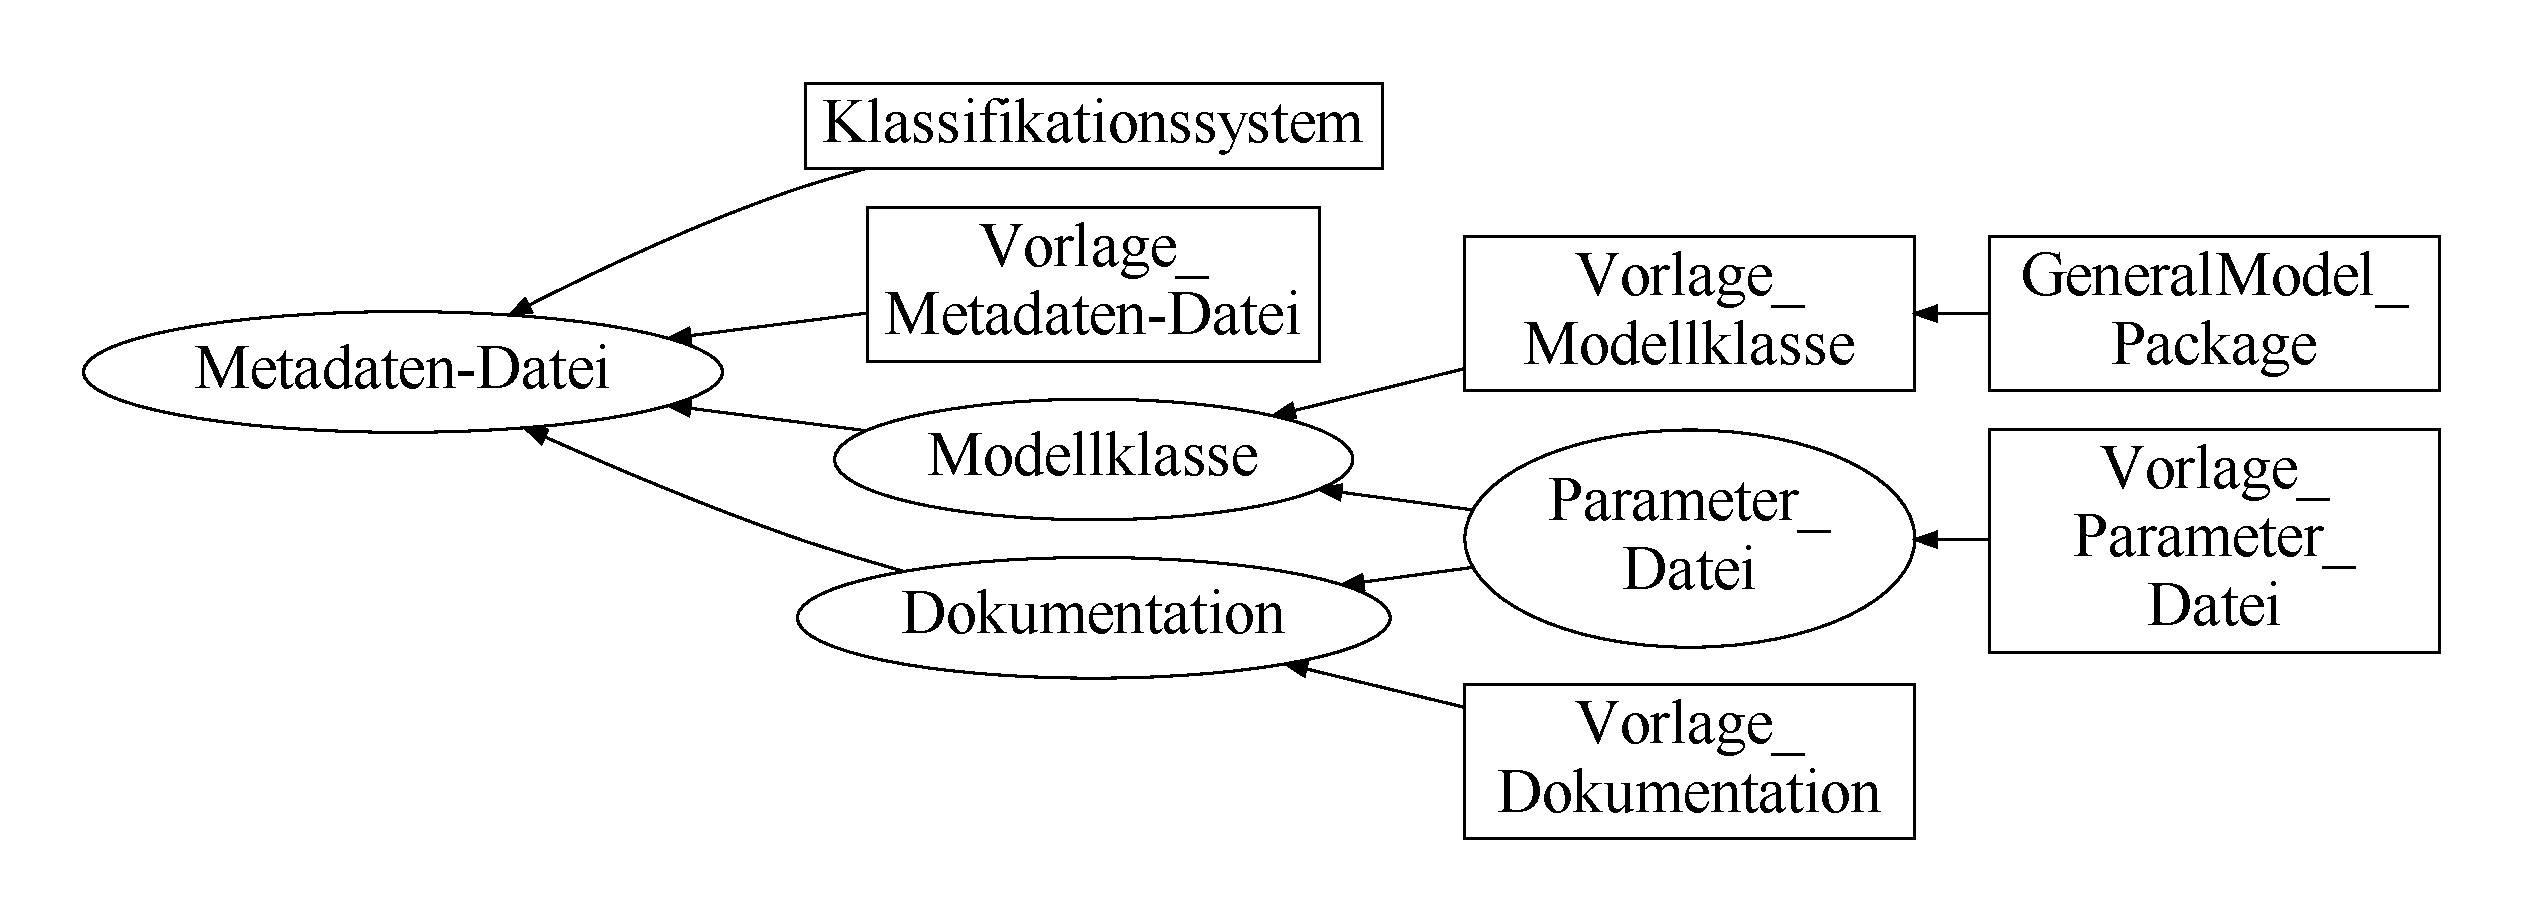
\includegraphics[width=1\linewidth]{Katalogstruktur}
	\caption[Katalogstruktur]{Elemente in Ellipsen existieren individuell für jedes Modell. Elemente in Rechtecken existieren genau ein Mal im Katalog.}
	\label{fig:Katalogstruktur}
\end{figure}

Das \textit{Klassifikationssystem} ist eine Übersicht der Modelleigenschaften und deren Beziehungen untereinander. Die Einträge in dem Feld für die Modelleigenschaften in der Metadaten-Datei(\textit{tag\_list}) sind nur Namen von Kategorieknoten aus dem KS. Es sorgt für eine einheitliche Namensgebung der Modelleigenschaften(s. Anforderung \ref{A.Modelleigenschaften}). 

Das Python Package \textit{GenericModel} stellt die Python Klasse \textit{GenericModel} zur Verfügung, von der alle Modellklassen der implementierten Modelle erben. Sie stellt ein Variablen- und Methodenset bereit, das alle Modellklassen gemeinsam haben.

Die \textit{Metadaten-Datei} ist eine Datei im YAML-Format, das Informationsfelder für Informationen zu dem zugehörigen Modell enthält. Es gibt Felder für Informationen\dots 
\begin{itemize}[label=$\bullet$]
	\item über das Modell (Modellname, Kurzbeschreibung, Modelleigenschaften, Dateinamen der Modellbilder)
	\item für eine Umsetzung des Kataloges als Datenbank(Key, Predecessor-Key, Implementation-Key)
	\item anderer Art (Modellersteller, Erstellungsdatum, Liste der Bearbeiter, Externe Referenzen)
\end{itemize}
Das Konzept und die Umsetzung der Metadaten-Datei stammt aus dem \textit{ACKRep}\footnote{ACKRep GitHub Repository: https://github.com/ackrep-org/ackrep\_data}. 
% Noch schreiben welche Informationen im aktuellen Stand gegeben werden?

Die \textit{Modelldokumentation} ist die textuelle Notation des Modells. Sie wird im \LaTeX-Format geschrieben. Nach jeder Bearbeitung wird die PDF-Datei aus der \LaTeX-Datei erzeugt. 

Die \textit{Parameter-Datei} ist eine Python-Datei. Diese enthält beispielhafte Parameterwerte für das Modell. Das Ausführen der Datei erzeugt eine Tabelle mit den beispielhaften Parameterwerten im \LaTeX-Format, schreibt diese in eine Datei Namens \textit{parameters.tex} und speichert die Datei im Ordner der Modelldokumentation. Außerdem stellt Sie eine Methode für die implementierte Modellklasse bereit, welche die Parameter des Modells als Rückgabewert hat.

Die implementierte \textit{Modellklasse} ist eine Python-Datei, welche das Modell als Python-Klasse enthält. 

Die \textit{Vorlagen} für die Metadaten-Datei, die Parameter-Datei, die Modelldokumentation und -implementation sind Dateien, welche den Arbeitsaufwand für das Anlegen neuer Modelle verringern sollen(siehe Entscheidung \ref{E.Vorlagen}). Die repetitiven Elemente für die entsprechenden Dateien sind in den Vorlagen schon vorhanden, so dass nur die Modellspezifischen Elemente neu geschrieben werden müssen. Die Verwendung der Vorlagen stellt eine einheitliche Struktur der Dateien sicher.

Die Ordnerstruktur des Kataloges liegt in einem Repository der Versionsverwaltungssoftware \textit{Git}\footnote{Der Katalog hat kein eigenes Repository, sondern liegt aktuell im Git-Repository dieser Studienarbeit. Deshalb wird an dieser Stelle kein Link zur Verfügung gestellt.}.  %TODO: Abschnitt zu Git in Vorbetrachtung

% =================================================
% ------------- Klassifikationssystem -------------
% =================================================
\section{Klassifikationssystem}
\label{Ch:Ergebnisse:Sec:KS}
Das \textit{Klassifikationssystem (KS)} stellt eine Wissensrepräsentation dar. Es lehnt stark an die in \cite{KNHE20a} eingeführte \textit{OCSE} an, von der es sich insofern unterscheidet, das im KS nur die Teilbereiche des Wissens der Mathematik, Regelungs- und Steuerungstheorie enthalten sind, die sich auf regelungstechnische Systeme und Modelle beziehen. Die im KS verwendeten Bezeichnungen sollen in den Metadaten-Dateien der Modelle bevorzugt verwendet werden. \\
Es ist anzumerken, dass das KS keine vollständige Wissensrepräsentation darstellt. Das liegt daran, dass das darzustellende Wissen sehr umfangreich ist und eine vollständige Darstellung dessen im Rahmen dieser Studienarbeit nicht schaffbar war. Weiter könnte man auch die Frage stellen, ob überhaupt eine vollständige Darstellung des beabsichtigten Wissensbereiches existiert, da das Wissen dynamisch mit neuen Entdeckungen wächst. Diese Diskussion soll hier aber nicht weitergeführt werden. 

Bei einem konkreten Modell im Katalog finden sich die Einträge des KS im Informationsfeld \textit{tag\_list} der Metadaten-Datei wieder. In diesem Informationsfeld werden die Modelleigenschaften und dessen Werte notiert, wobei für die Modelleigenschaften die Begriffe aus dem KS bevorzugt verwendet werden.Für die Einträge in der \textit{tag\_list} gilt eine Open-World Annahme. Wenn eine Eigenschaft nicht in der \textit{tag\_list} enthalten ist, dann enthält der Katalog keine Aussage darüber, ob das Modell die Eigenschaft besitzt oder nicht.

%TODO: Knotenanzahl einfügen
%TODO: Ausschnitt des KS einfügen
Das KS besteht aktuell aus <Knotenanzahl> Knoten. <Bildreferenz> zeigt ein Ausschnitt des KS.
% =============================================================
% ------------- Aufbau des Klassifikationssystems -------------
% =============================================================
\subsection{Aufbau des Klassifikationssystems}
\label{Ch:Ergebniss:Sec:KS:SubSec:Aufbau}
Das KS ist ein Semantisches Netz(s. \ref{E.KS_SemantischesNetz}), welches durch einen gerichteten, kreisfreien Graphen repräsentiert wird. Es gibt folgende Knotentypen: Kategorie-, Objekt-, Werte, und Wertetypknoten. 
Die Kanten zeigen Beziehungen zwischen den Knoten des KS auf, die durch die Kantenbeschriftungen spezifiziert werden. Es gibt folgende Kantennamen: \glqq is a\grqq, \glqq Value\grqq, \glqq Type\grqq und \glqq Object\grqq. Der Kantenname kennzeichnet zudem den Knotentyp des Startknotens der Kante. Jeder Endknoten einer Kante ist ein Kategorieknoten. Die Beziehung zwischen Knotentypen und Kantennamen wird in \autoref{table:KS_KantenUndKnoten} gezeigt.
\begin{table}[H]
	\centering
	\begin{tabular}{l|c|l}
		Startknotentyp & Kantenname & Endknotentyp \\ \hline
		Kategorieknoten & is a & Kategorieknoten \\
		Werteknoten & Value & Kategorieknoten \\
		Wertetypknoten & Type & Kategorieknoten \\
		Objektknoten & Object & Kategorieknoten
	\end{tabular}
	\caption{Beziehung zwischen Kantennamen und Knotentypen}
	\label{table:KS_KantenUndKnoten}
\end{table}

Die Kategorieknoten, außer der Ursprungsknoten und die Knoten der Hauptkategorien, können als Modellattribute interpretiert werden. In der Metadaten-Datei dürfen nur diese Knoten des KS eingetragen werden. \\
Die Kategorieknoten im KS werden durch ihren eindeutigen Namen identifiziert(s. \ref{E.KS_Namensgebung}).\\
Jeder Knoten $k$, außer der Ursprungsknoten, ist entlang eines gerichteten Pfades $P(k)$ mit dem Ursprungsknoten verbunden. Wird einem Modell ein Knoten $k_i$ des KS als Modellattribut zugewiesen, dann hat das Modell auch alle Knoten, außer Ursprungs -und Hauptknoten, entlang des gerichteten $P(k_i)$ als Modellattribut. Aus diesem Grund wird in der \textit{tag\_list} der Metadaten-Datei immer nur die spezifischste Eigenschafte eines Pfades angegeben. % Beispiel?

Der Ursprungsknoten \textit{Property\_Of\_Classification\_System} hat die drei Unterkategorien \textit{Property\_Of\_Mathematical\_Representation}, \textit{Model\_Behaviour} und \textit{Usage}. Die Unterkategorien des Ursprungsknoten werden im KS als Hauptkategorien bezeichnet, die jeweils verschiedene Teilmengen von Modellattributen enthalten. Die Hauptkategorien werden wie folgt Beschrieben.

\textbf{Eigenschaften der mathematischen Repräsentation}: \\
Umfasst Eigenschaften der mathematische Repräsentation des Modells.   % ... die aus der math. Rep. direkt hervor gehen. --> Äquivalenzbegriff von Willems

\textbf{Modelleigenschaften}: \\ % Eigenschaften unabhängig von Darstellungsform eines äquivalenten Systems
Umfasst Eigenschaften die aus der mathematischen Repräsentation mit Methoden der Regelungstechnik abgeleitet werden.

\textbf{Verwendung}: \\
Umfasst Aufgabentypen und Anwendungsbereiche in denen die Modelle häufig genutzt werden.

In \ref{Ch:Vorbetrachtung:Sec:SystemeModelle} wurde erwähnt, dass ein Modell mehrere mathematische Repräsentationen haben kann. Dieser Aspekt führt auf den Begriff der \textit{Äquivalenz} zweier mathematischer Modelle. Zwei mathematische Modelle heißen \textit{Äquivalent}, wenn beide das gleiche Set an Trajektorien für ihre externen Variablen zulassen\footnote{vgl. \cite{SCH89}, S. 34}. Oder einfacher, wenn beide Modelle das gleiche dynamische Verhalten aufweisen. Das Modell eines Systems kann durch eine Menge äquivalenter mathematischer Modelle repräsentiert werden. Der Unterschied zwischen den Hauptkategorien \textit{Eigenschaft der mathematischen Repräsentation} und \textit{Modelleigenschaften} liegt darin, dass die Elemente eine Menge äquivalenter mathematischer Modelle die gleichen \textit{Modelleigenschaften} haben, sich aber in ihrer mathematischen Repräsentation unterscheiden.

% ===========================================================================
% ------------- Technische Umsetzung des Klassifikationssystems -------------
% ===========================================================================
\subsection{Technische Umsetzung des Klassifikationssystems}
\label{Ch:Ergebnisse:Sec:KS:SubSec:TechUmsetzung}
Das KS wird technisch mit vier Dateien im YAML-Format realisiert, welche folgende Namen haben: \textit{KS\_Tree\_main}, \textit{KS\_Tree\_Math\_Representation}, \textit{KS\_Tree\_Model\_Attributes} und \textit{KS\_Tree\_Usage}. Die Datei \textit{KS\_Tree\_main} enthält die \textit{Informationsblöcke(IB)} zu dem Ursprungsknoten und den Knoten der Hauptkategorien. Die restlichen drei Dateien enthalten jeweils die Informationsblöcke zu den Knoten der Unterkategorien der Hauptkategorien. \\ 
Ein IB enthält alle Informationen zu genau einem Knoten des KS. Jeder IB in den YAML-Dateien ist ein Mapping. Ein Mapping setzt einen Schlüssel mit genau einem Wert in Beziehung. Das \textit{dictionary} ist das Python-Äquivalent zu einem Mapping. In jedem IB ist der Name des Knotens der Schlüssel und eine Sequenz ist der Wert. \textit{List} und \textit{tuple} sind die Python-Äquivalente zur Sequenz. Jeder Eintrag der Sequenz steht für ein Attribut des Knotens und ist wiederum ein Mapping, dessen Schlüssel der Attributsname und dessen Wert der Attributswert ist. Die IB\grq s sind durch eine Leerzeile voneinander getrennt. Die Abbildung <Abbildungsreferenz> zeigt einige IB\grq s aus der Datei \textit{KS\_Tree\_Math\_Representation}.\\ %TODO: Beispielbild IB's hinzufügen
Eine Kante wird durch die Elemente \textit{Pre\_Node} und \textit{Edge\_Name} definiert. Diese stehen jeweils als Einträge in der Sequenz des Informationsblocks des Startknotens der Kante.

Zusätzlich gibt es das Python-Skript \textit{KS\_Create\_Graph}, welches die YAML-Dateien mit Hilfe des Packages \textit{pyyaml}\footnote{Pyyaml Package: https://pyyaml.org/wiki/PyYAMLDocumentation} einliest. Zudem erzeugt es einen gerichteten Graphen des Python Packages \textit{networkx}\footnote{Networkx Package: https://networkx.org/documentation/stable/index.html} und zeichnet den Subgraphen, der nur die Kategorieknoten, enthält mit dem Python Package \textit{nxv}\footnote{Nxv Package: https://nxv.readthedocs.io/en/latest/index.html} in eine Bilddatei.

Ein gerichteter Graph des networkx-Packages besteht aus einer Menge von Knoten und Kanten. Zu jedem Knoten und jeder Kante kann eine beliebig große Menge individuell benannter Attribute hinzugefügt werden. So werden z.\,B. die Kantennamen der entsprechenden Kante als Attribut hinzugefügt. Die Wertetypknoten sind als Attribut eines Kategorieknotens implementiert. Diese Umsetzung des implementierten Graphen ist aus technischer Sicht sinnvoll, da die Information über die Attribute eines Knotens so intuitiver zu erreichen sind. Es soll hier jedoch erwähnt werden, das diese Implementierung von einer korrekten Darstellung des KS als Semantisches Netz abweicht, da Kategorieknoten nur explizite, als Knoten aufgeführte Attribute besitzen. Für eine formal korrekte Implementierung des KS als Semantisches Netz müssten Knoten welche die Attribute einer Kategorie darstellen auch explizit als Knoten angelegt werden.\\
Die gewählte Implementierung des KS ist einfach erweiterbar und bearbeitbar. Eine Veränderung im Umfang des KS, also das Hinzufügen neuer Knoten zum KS oder das entferne von Knoten aus dem KS, wird in der Implementierung durch schreiben neuer IB\grq s oder entfernen von IB\grq s erreicht. Sollen neue Knotentypen zum KS hinzugefügt werden z.\,B. Referenzknoten, welche eine Referenz zur Definition der Kategorie enthalten würden, so werden diese als neuer Eintrag zu den Sequenzen der IB\grq s hinzugefügt.

%TODO: Vllt eher in Ausblick?
Die Implementierung des KS ist auch relativ einfach für eine potenzielle Integration einer Suchfunktion zu öffnen, indem zu dem Python-Skript \textit{KS\_Create\_Graph} eine Methode hinzugefügt wird, welche die networkx-Graphen des KS als Rückgabewert liefert.  
% Networkx-Graphen vom Funktionsumfang potenziell als vollständige maschinelle lesbare Repräsentation des KS und dessen Anwendungen auf die Modelle verwendbar

% ===============================================
% ------------- Modelldokumentation -------------
% ===============================================
\section{Modelldokumentation}
\label{Ch:Ergebnisse:Sec:Dokumentation}
Die Modelldokumentation enthält die textuelle Notation des Modells in einer Datei im \LaTeX-Format. Die Dokumentation besteht aus den Abschnitten: \textit{Nomenklatur}, \textit{Modellgleichungen}, \textit{Herleitung und Erklärungen} und \textit{Referenzen}. Der Abschnitt \textit{Herleitung und Erklärung} ist optional.

\textbf{Nomenklatur}:\\
Die Nomenklatur enthält alle in der Dokumentation genutzten Variablen und eine Beschreibung, für welche Größen diese stehen. Die Nomenklatur ist aufgeteilt in die Sektionen \textit{Nomenklatur für die Modellgleichungen} und \textit{Nomenklatur für die Herleitung}. Die \textit{Nomenklatur für die Modellgleichungen} enthält die Variablen, die im gleichnamigen Abschnitt verwendet werden und muss in jeder Dokumentation enthalten sein. Die \textit{Nomenklatur für die Herleitung} enthält alle Variablen die für den Abschnitt \textit{Herleitung und Erklärung} genutzt werden, bis auf die Variablen die in der Sektion \textit{Nomenklatur für die Modellgleichungen} schon enthalten sind. Die \textit{Nomenklatur für die Herleitung} ist nur zu schreiben, wenn der Abschnitt \textit{Herleitung und Erklärung} existiert. %TODO: Beispielnomeklatur (MMC oder Boost converter) einfügen

\textbf{Modellgleichungen}:\\
Der Abschnitt \textit{Modellgleichungen} besteht aus einer formalisierten Darstellung der Modellgleichungen und weiteren Sektionen, die gleich noch benannt werden. Die formalisierte Darstellung der Modellgleichungen besteht aus drei Teilen.  
\begin{itemize}[label=$\bullet$]
	\item einer Zuordnung der Variablen zum generalisierten Zustands-, Eingangs- und (optional) Ausgangsvektor
	\item einem Gleichungssystem von Differentialgleichungen erster Ordnung(s. \ref{E.Textdok}), das die generalisierten Zustands- und Eingangsvariablen verwendet
	\item der Benennung, welche Variablen Parameter sind
\end{itemize} %TODO: Beispiel Modellgleichungen
Die weiteren Sektionen sind recht frei gestaltbar und sollen weitere nützliche Informationen zu dem Modell liefern. Aktuell sind in der Vorlage nur die Sektionen \textit{Annahmen} und \textit{Beispielhafte Parameterwerte} explizit formuliert. Weitere Sektionen können vom Ersteller des Modells nach eigener Einschätzung der Sinnhaftigkeit hinzugefügt werden. Denkbar wäre, angenommen es handelt sich um ein flaches Modell, z.\,B. ein Abschnitt der flache Ausgänge benennt. Die Sektion \textit{Beispielhafte Parameterwerte} ist als einzige unter den weiteren Sektionen zwingend zu füllen. Dies geschieht mehr oder weniger automatisch, da die Datei \textit{paramters.tex}, die durch die \textit{Parameter-Datei} erstellt wird, dafür eingebunden wird.

\textbf{Herleitung und Erklärungen}:\\
Dieser Abschnitt ist für die Dokumentation optional. Er soll die Möglichkeit bieten die Herleitung des Modells zu beschreiben oder weitere aus Sicht des Modellerstellers sinnvolle Erklärungen zu liefern.

\textbf{Referenzen}:\\
Enthält die Referenzen, die für die Erstellung der Modelldokumentation verwendet wurden.

Aus der \LaTeX-Datei der Modelldokumentation wird eine für Menschen gut lesbare PDF-Datei erzeugt. 

% =================================================
% ------------- Modellimplementation  -------------
% =================================================
\section{Modellimplementation}
\label{Ch:Ergebnisse:Sec:Implementation}
Modelle des Kataloges werden in Form einer Python-Klasse implementiert. Bei Initialisierung eines Objektes der Modellklasse können dem Konstruktor die Zustandsdimension, eine Eingangsfunktion und ein Parametervektor übergeben werden. Alle dieser Variablen haben Standardwerte. Jede Modellklasse bezieht ein Standardset von Parameterwerten aus der \textit{Parameter-Datei} (die Standardparameter sind also identisch mit den beispielhaften Parameterwerten aus der Dokumentation) und hat eine Standardfunktion für die Modelleingänge integriert.\\ 
Ein Modell kann also einfach über ein eigens erstelltes Python-Skript simuliert werden(vgl. \ref{A.Implementierung}), indem eine Objekt der Modellklasse erzeugt wird, ein Startvektor für den Modellzustand definiert wird und anschließend das Modell mit einer geeigneten Methode(z.\,B. \textit{solve\_ivp} des Packages \textit{scipy}) simuliert wird. Die Methode \textit{get\_rhs\_func} der Modellklasse stellt die dafür benötigte Python-Funktion zur Verfügung.

Die Parameter und die Eingangsfunktion eines Modellobjektes können nach Initialisierung mit den Methoden \textit{set\_parameters} und \textit{set\_input\_func} geändert werden. Die Zustandsdimension ist nur bei Initialisierung einstellbar und das auch nur bei Modellen, deren Zustandsdimension nicht festgelegt ist(z.\,B. beim N-Fach-Integrator).\\
Die Methode \textit{get\_rhs\_symbolic} liefert die symbolischen Modellgleichungen als Rückgabewert. Zur Implementierung der symbolischen Gleichungen wird das Python-Package \textit{sympy} verwendet.

%Obsoloter Absatz?
Jede Modellklasse erbt von der Klasse \textit{GenericModel}, welche eine Menge von Methoden und Variablen definiert, die jede Modellklasse haben muss. Die Methoden, die nicht für jede individuelle Modellklasse angepasst werden müssen sind in der Klasse \textit{GenericModel} implementiert.\\
Innerhalb einer Modellklasse sind nur die symbolischen Gleichungen als Code geschrieben. Die Umwandlung in die numerischen Form erfolgt in der Methode \textit{get\_rhs\_func} mit der Methode \textit{lambdify} des Sympy-Packages.\\
% Hinweis das bei Codesyntax versucht wurde nach PEP8 zu arbeiten?

Mittels der aktuellen Vorlagen können nur Modelle, deren Verhalten durch gewöhnliche Gleichungssysteme erster Ordnung beschrieben wird, implementiert werden.

% ==============================================
% ------------- Vorhandene Modelle -------------
% ==============================================
\section{Vorhandene Modelle}
\label{Ch:Ergebnisse:Sec:Modelle}

% ==============================================
% ------------- Katalogerweiterung -------------
% ==============================================
\section{Katalogerweiterung}
\label{Ch:Ergebnisse:Sec:Erweiterung}
Die letzte Anforderung an den Katalog war, das dieser erweiterbar sein soll (Anforderung \ref{A.Erweiterbarkeit}). In diesem Abschnitt wird beschrieben, welche Schritte für die Erweiterung des Kataloges nötig sind. 

Der Katalog wird über das Hinzufügen neuer Modelle erweitert. Wir nehmen an, dass die Recherche für das hinzuzufügende Modell abgeschlossen ist. Damit ist gemeint, dass die nötigen Informationen zu dem Modell wie Modellgleichungen, beispielhafte Parameterwerte, Beschreibung der Variablen und die dazugehörigen Referenzen schon bekannt sind. Zudem wird angenommen, das der Modellersteller sich mit der Ordnerstruktur des Kataloges vertraut gemacht hat.\\

Zuerst muss das Git-Repository des Kataloges heruntergeladen werden, um eine lokale Kopie des Kataloges und der Vorlagen(siehe Abschnitt \ref{Ch:Ergebnisse:Sec:Struktur} \nameref{Ch:Ergebnisse:Sec:Struktur}) zu erhalten. Danach muss ein Ordner für das neue Modell und ein Ordner für dessen Implementation erstellt werden. Anschließend muss die Metadaten-Datei, die Modelldokumentation und die Parameter-Datei mithilfe der Vorlagen erstellt werden.\\
Für die \textit{Metadaten-Datei} wird die Vorlage in den Modellordner kopiert und in \textit{metadata.yml} umbenannt. Danach sind die Informationsfelder, wie Name, Autor, Kurzbeschreibung etc. zu füllen. 
Das erschließen der Modelleigenschaften für die \textit{tag\_list} wird dabei voraussichtlich die meiste Zeit in Anspruch nehmen.\\
Ebenso wird für die \textit{Modelldokumentation} die entsprechende \LaTeX-Vorlage zuerst in den Modellordner kopiert und dann ausgefüllt. Für das Einfügen der Modellgleichungen müssen diese in ein Gleichungssystem von Differentialgleichungen erster Ordnung überführt werden.\\
Bevor die PDF-Datei der Modelldokumentation erzeugt werden kann, wird die \LaTeX-Datei mit den beispielhaften Parameterwerten benötigt. Diese wird durch die \textit{Parameter-Datei} erzeugt. Um die Parameter-Datei anzufertigen wird die zugehörige Vorlage in den Ordner der Modellimplementation kopiert und entsprechend ausgefüllt. Danach wird die Parameter-Datei ausgeführt\footnote{Zur Erinnerung: Die Parameter-Datei ist ein Python Skript.}. Jetzt kann die PDF-Datei der Modelldokumentation erzeugt werden. Anschließend kann die \textit{Pull-Request}, eine Anfrage für das Zusammenfügen des lokalen Kataloges mit dem Repository des Kataloges, erfolgen.

Die Implementierung eines Modells ist zwar optional(siehe Entscheidung \ref{E.ImplementierungOptional}) aber in jedem Falle erwünscht und soll hier für Modelle, deren Verhalten ausschließlich durch Differentialgleichungen erster Ordnung beschrieben wird, erläutert werden. Die Implementierung eines Modells erfolgt durch das erstellen der \textit{Modellklasse}. Dafür wird die entsprechende Vorlage in den Ordner der Modellimplementation kopiert und die mit dem Kommentar \glqq Model Dependent\grqq gekennzeichneten stellen ausgefüllt. Die Validierung der Modellklasse muss durch ein komplett eigenständig erstelltes Python-Skript erfolgen. Die Test-Dateien anderer implementierter Modelle können dafür als Orientierung verwendet werden.



